\begin{exercise}
  Describe, in simple sentences with a minimum of mathematical formalism, (1) the score
  of a graph, (2) what the graph score theorem is, (3) the idea of the 
  graph score algorithm, (4) where the difficult part of its proof is.
  Imagine you have a friend who does not take this class, and think about how to answer
  the above questions to them.
\end{exercise} 

\textbf{Theorem}
\par Let $d=(d_1,\cdots,d_n)$ with $d-1\le\cdots\le d_n$. Define $d'$ by
\begin{center}
$$ d_i'=\left\{
\begin{array}{rcl}
d_i-1       &      & {i=n-d_n,\cdots,n-1,n}\\
d_i         &      & {i=1,\cdots,n-d_n-1}\\
\end{array} \right. $$
\end{center}
\par Then there exists a graph with score $d$ if and only if there exist a graph with score $d'$
\par Furthermore, if $n=1$, then there exist a graph with score $(d_1)$ if and only if $d_i=1$.
\textbf{Idea of Algorithm}
\par find-graph $(d_1,d_2,\cdots,d_n)$
\par sort$(d_1,d_2,\cdots,d_n)$
\begin{center}
$$ d_i'=\left\{
\begin{array}{rcl}
d_i-1       &      & {i=n-d_n,\cdots,n-1,n}\\
d_i         &      & {i=1,\cdots,n-d_n-1}\\
\end{array} \right. $$
\end{center}
\par $G'=$ find-graph$(d_1',d_2',\cdots,d_{n-1}')$
\par if $G'=$ NULL
\par return NULL
\par else $G=G'+vertex(n)$
\begin{figure}[hpbt]
\begin{center}
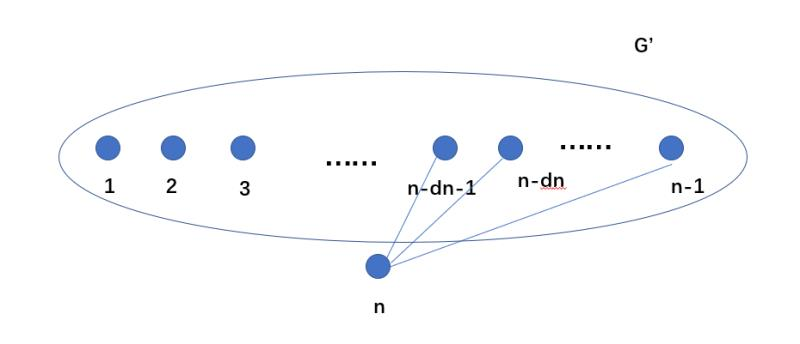
\includegraphics[width = 0.8 \textwidth]{score.png}
\end{center}
\end{figure}
\textbf{Trying to explain it over lunch:}
\par We sort the degree in a non-decreasing order. Every time we eliminate the vertex with the largest degree(suppose it is $x$). We subtract 1 from the other $x^{th}$ largest degree of the vertices. If we succeed in doing it until the end with no negative numbers. We succeed in finding the graph.



